\chapter{Week 6: Arduino met Pi Koppelen}

In deze laatste week van het vak Programmeren 2, gaan we ons eerst nog wat verder verdiepen in de wereld van object geörienteerd programmeren (OOP). Daarnaast stevenen we af op onze eindopdracht van dit vak.

\section{Overerven}\index{Overerven}
Met het vorige hoofdstuk heb je je eerste introductie gehad in de wereld van OOP. We hebben op een nieuwe abstracte manier naar problemen gekeken. Ook werd er toen verteld over de voordelen van OOP, zo kon je de code makkelijk onderhouden (je hoeft maar op $1$ plek de klasse-definitie/blauwdruk aan te passen, en overal waar je 'm gebruikt wordt deze verandering overgenomen). Maar ook werd er gesteld dat de gemaakte code eenvoudig uitbreidbaar is, en op dat voordeel hebben we nog niet naar gekeken. Als we nu ons geheugen opfrissen door even te kijken naar de gemaakte \pyth{Cirkel}-klasse:

\inputpython{code/chapter08/cirkel.py}

We hadden een klasse \pyth{Cirkel} gemaakt die als eigenschap z'n straal had, en waarop we de functies \pyth{bereken_oppervlakte()} en \pyth{bereken_omtrek()} op kunnen uitvoeren. We kunnen nu deze klasse-definitie nu ook gebruiken om andere klasse te definiëren die gebasseerd zijn op deze cirkel. \newline 

Als we bijvoorbeeld een klasse willen maken voor een \pyth{Bol} en we gaan hiervoor beredeneren wat zijn eigenschappen en z'n functies zijn. Zul je zien dat deze veel zullen overeenkomen met die van de \pyth{Cirkel}. Qua eigenschappen kunnen we een bol definieren op basis van een straal en op basis van die straal kunnen we de omtrek, oppervlakte en inhoud van de bol berekenen. Grafisch weergegeven:
\begin{figure}[h!]
\centering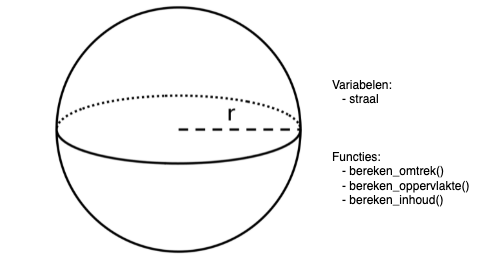
\includegraphics[scale=0.7]{Pictures/chapter08/bol.png}
\caption{\small Ons bol-object heeft een straal, en kan (op basis daarvan) de omtrek, oppervlakte en inhoud van zichzelf berekenen.}
\label{fig:bol} % Unique label used for referencing the figure in-text
%\addcontentsline{toc}{figure}{Figure \ref{fig:webserver}} % Uncomment to add the figure to the table of contents
\end{figure}

Zowel de klasse-variabele \pyth{r}, als $2$ van de $3$ functies\footnote{Wellicht heb je 'm al door: de oppervlakte van een bol berekenen je op een andere manier dan van een cirkel, hier komen we later op terug} komen overeen met die van \pyth{Cirkel}. Als we dus een klasse-definitie voor een \pyth{Bol} willen maken is het handiger om deze te baseren op \pyth{Cirkel} dan helemaal opnieuw te beginnen, dat scheelt werk! Onze klasse-definitie van een \pyth{Bol} ziet er dan zo uit:

\inputpython{code/chapter08/bol.py}

Valt het je op hoe kort dit bestand is? Op regel $5$ gebeurt alle 'magie', hier wordt namelijk gesteld dat we een nieuwe klasse genaamd \pyth{Bol} willen maken, maar dat we deze willen baseren op \pyth{Cirkel}. \textit{Python} regelt nu onderwater dat de bol-klasse een klasse-variabele \pyth{r} voor de straal krijgt, en ook kan hij gebruik maken van de functies (waaronder de constructor) die in \pyth{Cirkel} zitten. \newline

Het enige wat wij zelf nog moeten doen is de nieuwe functie uitschrijven die de inhoudt van de bol berekend op basis van z'n straal, met de volgende formule: $V_{bol} = \frac{4}{3} \pi r^3$. \newline

\begin{remark}
  Een klasse basseren op een andere klasse noemen we ook wel een \textit{subklasse} maken. \pyth{Bol} is in dit geval een \textit{subklasse} van \pyth{Cirkel}. Andersom is \pyth{Cirkel} de \textit{superklasse} van \pyth{Bol}.
\end{remark}

Deze klasse-definitie kunnen we daarna gebruiken in andere programma's op de bekende manier:
\begin{python}
from bol import Bol

mijn_bol = Bol(10)  # Maak een bol aan met een straal van 10.

omt = mijn_bol.bereken_omtrek()
opp = mijn_bol.bereken_oppervlakte()
inh = mijn_bol.bereken_inhoud()

print(f"Omtrek: {omt:.2f}")
print(f"Oppervlakte: {opp:.2f}")
print(f"Inhoud: {inh:.2f}")
\end{python}

Wat het onderstaande als uitvoer geeft:
\begin{python}
Omtrek: 62.83
Oppervlakte: 314.16
Inhoud: 4188.79
\end{python}

We maken hier een object genaamd \pyth{mijn_bol} aan, die van het type \pyth{Bol} is. Doordat onze Bol klasse-definitie geen constructor heeft, wordt de constructor van z'n superklasse aangeroepen: die van \pyth{Cirkel}. Daarna worden de functies \pyth{bereken_omtrek()} en \pyth{bereken_oppervlakte()} aangeroepen. Deze zijn ook niet te vinden in de \pyth{Bol} klasse-definitie, dus worden die van \pyth{Cirkel} hier uitgevoerd. De laatste functie \pyth{bereken_inhoud()} is wel te vinden in \pyth{Bol}, dus die wordt aangeroepen zoal we gewend zijn. \newline

Python zoekt dus eerst in de klasse-definitie van een subklasse naar klasse-variabelen en functies, en als ze daar niet te vinden zijn kijkt hij naar de superklasse ervan. (zijn ze daar ook niet vinden, dan krijg je een \pyth{AttributeError} ;) ). \newline

In onze \pyth{Bol} zit echter nog wel een bug, de oppervlakte van een bol, bereken je op een andere manier dan van een cirkel. Voor een cirkel geldt: $O_{cirkel} = \pi r^2$, voor een bol: $O_{bol} = 4\pi r^2$. \newline

Gelukkig kunnen we in een subklasse functies van de superklasse makkelijk overschrijven:
\inputpython{code/chapter08/bol2.py}

Als we nu onze \pyth{Bol} gebruiken, zoals boven aan deze pagina, komen er wel de juiste waardes uit:
\begin{python}
Omtrek: 62.83
Oppervlakte: 1256.64
Inhoud: 4188.79
\end{python}

In dit geval zoekt Python eerst naar de functie \pyth{bereken_oppervlakte()} in \pyth{Bol}, en vindt 'm daar al, hij zoekt dan niet meer verder. Op deze manier kun je dus functies 'vervangen' van de superklasse in de subklasse. \newline \newline

We doen nog een voorbeeldje. Want we kunnen het overerven ook andersom benaderen. Stel je voor je wil op een OOP manier een kat, een hond en een koe beschrijven. In dit voorbeeld heeft elk dier een aantal variabelen en een aantal functies: 

\begin{figure}[h!]
\centering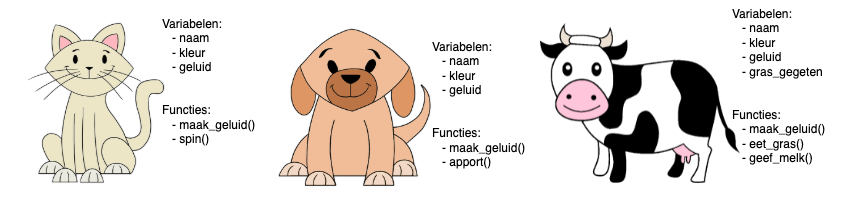
\includegraphics[scale=0.5]{Pictures/chapter08/animals.png}
  \caption{\small Elk dier (kat, hond en koe) heeft z'n eigen eigenschap en functies.} 
\label{fig:animals} % Unique label used for referencing the figure in-text
%\addcontentsline{toc}{figure}{Figure \ref{fig:webserver}} % Uncomment to add the figure to the table of contents
\end{figure}

Deze zou je nu los van elkaar gaan uit kunnen werken in code, maar je kunt ook eerst kijken naar de overeenkomsten. Deze overeenkomsten zou je namelijk kunnen verzamelen in een basis superklasse (bijv. 'dier') , waarop je de andere dieren op basseert. \newline

\begin{figure}[h!]
\centering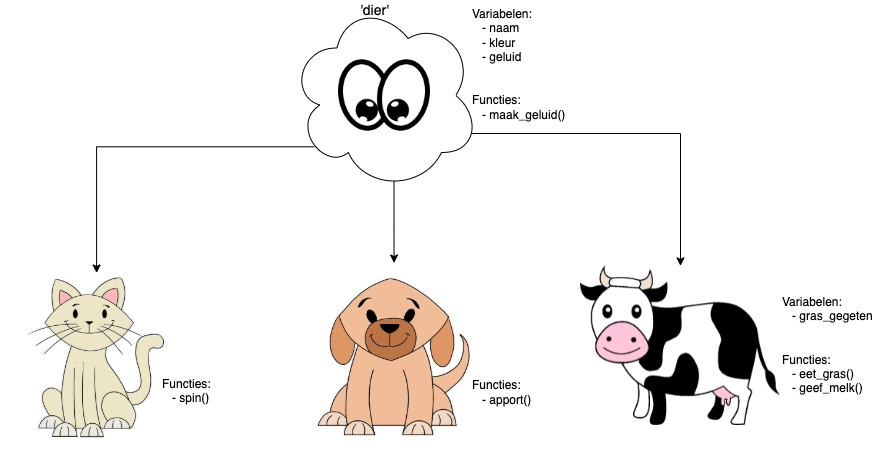
\includegraphics[scale=0.5]{Pictures/chapter08/animals_inh.png}
  \caption{\small Elk dier (kat, hond en koe) heeft z'n eigen eigenschap en functies, maar ook veel overeenkomsten met de basisklasse.} 
\label{fig:animals2} % Unique label used for referencing the figure in-text
%\addcontentsline{toc}{figure}{Figure \ref{fig:webserver}} % Uncomment to add the figure to the table of contents
\end{figure}

Laten we dit eens uit gaan werken in code. In de klasse-definitie van het basis-Dier (\textit{dier.py}), vinden we dus de \pyth{naam}, de \pyth{kleur} en het \pyth{geluid} dat het dier maakt. Ook zit hierin een functie \pyth{maak_geluid()} die het geluid van het dier op het scherm print:

\newpage

\inputpython{code/chapter08/dier.py}
In de overige dieren hoeven we dus alleen de functies en variabelen uit te werken die niet in de superklasse \pyth{Dier} zitten. Voor het gemak hebben we ze alledrie in hetzelfde bestand gezet: 
\inputpython{code/chapter08/dieren.py}

In de constructor van elk dier gebeurt nog iets bijzonders. Hier wordt namelijk met de hand de constructor van de superklasse \pyth{Dier} aangeroepen. Op deze manier worden alle klasse-variabelen met de goede waarde gezet. Nu kunnen we onze gemaakte dieren gebruiken:
\inputpython{code/chapter08/dieren_use.py}
De uitvoer laat zich raden (met toegevoegde witregels):
\begin{python}
Miauw!
Waf woef!
Mmmmmmboe!

Purrrrrr...

Bal! Bal! Bal!

Eerst gras eten..
Om nom nom
Hier, alsjeblieft: 1 melk!
\end{python}

\begin{remark}
  Wat nu als we een functie proberen uit te voeren van een ander dier? \newline 
  Bijv.: \pyth{bertha7.spin()}. Dan krijg je een error: \newline
  \pyth{AttributeError: 'Koe' object has no attribute 'spin'}.\newline
  De klasses die afgeleid zijn van een superklasse hebben geen weet van andere afgeleide klasses.
\end{remark}

\newpage

\section{Protocollen}\index{Protocollen}
Genoeg over abstracte concepten als OOP gehad. Tijd om eens te gaan verdiepen in hoe we onze Raspberry Pi en onze Arduino met elkaar kunnen laten communiciëren. Dit kan op verschillende manieren, beide hebben een vrij uiteenlopend scala aan communicatie mogelijkheden aan boord. We gaan in dit vak aan de slag met twee: via de seriële poort (ook wel: UART) en via Ethernet.

\subsection{UART}\index{UART}
Communicatie via UART of seriële poort wordt op de beide bordjes geregeld door de usb-poort. Je kunt ook bepaalde pinnen op de headers gebruiken, maar gemakshalve blijven we in dit hoofdstuk bij de usb-poorten.

\begin{figure}[h!]
\centering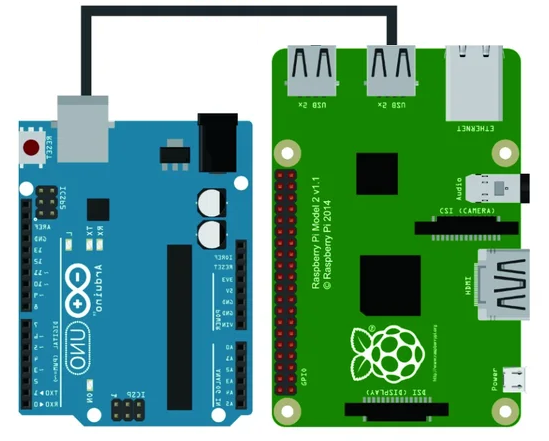
\includegraphics[scale=0.5]{Pictures/chapter08/usb.png}
  \caption{\small De \textit{Raspberry Pi} gekoppeld aan de \textit{Arduino} met een USB kabel.} 
\label{fig:usb} % Unique label used for referencing the figure in-text
%\addcontentsline{toc}{figure}{Figure \ref{fig:webserver}} % Uncomment to add the figure to the table of contents
\end{figure}

\begin{exercise}
  Sluit de \textit{Arduino} via USB aan op de \textit{Raspberry Pi}.
\end{exercise}
Onder Windows is de seriële poort, zoals je weet, te vinden als COM\textit{X}, waarbij \textit{X} een letter is (\textit{COM1}, \textit{COM5}, etc.). Omdat er op onze \textit{Raspberry Pi} een Linuxvariant (Raspberry Pi OS) draait, is het verstandig om even stil te staan bij hoe de seriële poort daar werkt.\newline

\newpage 

\subsection{Seriële poort in Linux}
Linux zit nogal anders in elkaar dan Windows. De menubalk die ineens bovenin zit, is het eerste wat in het oog schiet, maar dat is slechts het topje van de ijsberg. Wellicht heb je wel eens een file-explorer gestart, en dan zag het volgende: 
\begin{figure}[h!]
\centering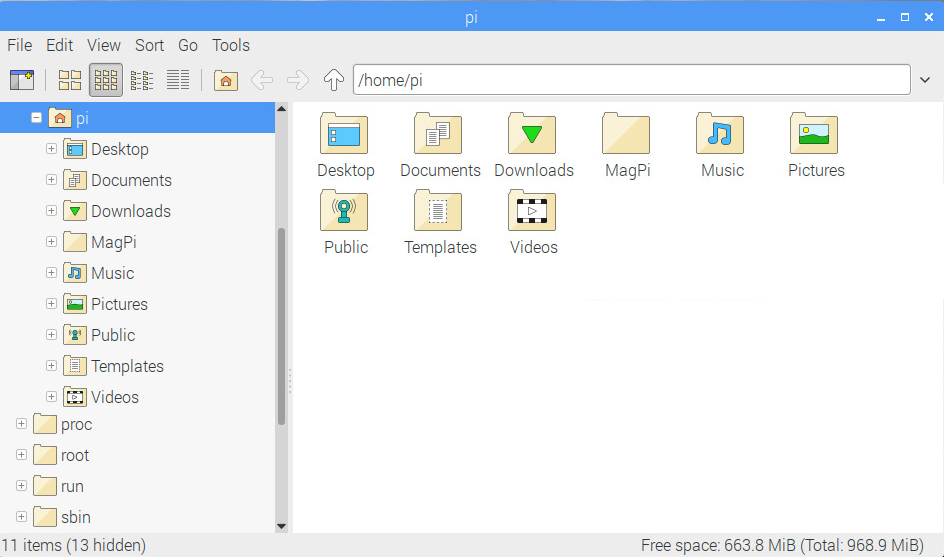
\includegraphics[scale=0.35]{Pictures/chapter08/home_folder.png}
  \caption{\small De home folder map met de bekende folders} 
\label{fig:home_folder} % Unique label used for referencing the figure in-text
%\addcontentsline{toc}{figure}{Figure \ref{fig:webserver}} % Uncomment to add the figure to the table of contents
\end{figure}

Dat komt waarschijnlijk redelijk bekend voor, de \textit{home} folder (voor de gebruiker \textit{pi}) lijkt nog redelijk op de folder \textit{Mijn Documenten} op Windows. Maar ga nu eens twee mapjes hoger. Je kom nu uit bij de zogeheten \textit{root-folder}, aangegeven met: '\textit{/}'. Deze is vergelijkbaar met de \textit{C:} schijf onder Windows. 
Waarschijnlijk vraag je je af wat dit allemaal voor vreemde folder zijn, en waar zit dan bijv. Linux geïnstalleerd er is namelijk geen '\textit{/linux}'-folder (zoals er onder windows wel een '\textit{C:\textbackslash Windows}'-folder is). Tja, dat is dus compleet anders hier. We gaan er niet te diep op in (want dat is een vak an sich), maar een beetje kennis ervan is wel handig als je hardware wil aansturen/uitlezen zoals de seriële poort.\newline

Onder Linux is 'alles een bestand'. Dus niet alleen je je standaard tekst-bestanden, plaatjes, video's etc. maar alles. Dus bijv. alle programma's die je draait zijn te vinden onder de '\textit{/proc}'-folder (het tooltje \textit{top} en \textit{htop} halen bijv. hier al hun informatie weg). Informatie over de computer zelf (zoals het aanwezige geheugen en de CPU) kun je vinden in \textit{/sys}. En alle aangesloten hardware zijn te vinden onder \textit{/dev} (van devices). 

Bijv. je harde schijf zit hier (in het geval van de Pi, als \textit{/dev/mmcblk0}). Heb je een muis aangesloten? Dan is die te vinden hier als \textit{/dev/input/mouse0}. De aangesloten \textit{Arduino} is hier ook te vinden. De vraag is alleen welk bestand moet ik hiervoor hebben? \newline

Het handige daarvoor is om de \textit{Arduino} even los te koppelen en een terminal te openen op de \textit{Pi}. Typ nu het volgende in:
\begin{lstlisting}[language=bash]
ls /dev/tty*
\end{lstlisting}
Dit geeft een (flinke) lijst met apparaten. Sluit nu de \textit{Arduino} weer aan en voer de bovenstaande regel opnieuw uit. Het apparaat wat er nu bij gekomen is, is de \textit{Arduino}. Onthou deze.

\begin{remark}
  De \textit{Arduino} zal waarschijnlijk zitten op \textit{/dev/ttyUSB0} of \textit{/dev/ttyACM0}.
\end{remark}

\newpage 

\subsubsection{Arduino code: Schrijven naar seriële poort}
Om de seriële poort uit te lezen zijn is het natuurlijk wel handig dat de \textit{Arduino} daar iets mee doet. We maken even snel een klein programmaatje op de Arduino die precies dat doet en laden dat erop:
\begin{lstlisting}[language=Arduino, basicstyle=\ttfamily\footnotesize]
void setup() 
{
  Serial.begin(9600);
}

void loop() 
{
  Serial.println("Hallo vanaf Arduino!");
  delay(1000); // Wacht een seconde.
}
\end{lstlisting}
\begin{exercise}
  Laad het bovenstaande programma op je \textit{Arduino}. Je kunt 'm ook gewoon programmeren op de \textit{Pi} door daar de Arduino-IDE te gebruiken. Is hij toch nog niet geïnstalleerd? Dan:
  \begin{lstlisting}[language=bash]
  sudo apt install arduino
  \end{lstlisting}
\end{exercise}

\subsection{PySerial}

\begin{figure}[h!]
\centering
\includegraphics[scale=0.75]{Pictures/chapter08/pyserial.png}
\label{fig:pyserial} % Unique label used for referencing the figure in-text
%\addcontentsline{toc}{figure}{Figure \ref{fig:webserver}} % Uncomment to add the figure to the table of contents
\end{figure}

Tijd om te kijken of we de data die nu gestuurd wordt door de \textit{Arduino} kunnen lezen met de \textit{Pi} via \textit{Python}. Dit gaan we doen met een handige package genaamd \textit{PySerial}. 

\begin{remark}
  Als het goed is, is deze package standaard geïnstalleerd op de \textit{Pi}, zoniet dan even onderstaande uitvoeren in een terminal:
  \begin{lstlisting}[language=bash]
    python3 -m pip install pyserial
  \end{lstlisting}
\end{remark}

Onderstaande stuk code is alles wat we hiervoor nodig hebben:
\inputpython{code/chapter08/arduino_serial.py}

We maken hierin een object genaamd \pyth{ser} aan, van het type \pyth{serial.Serial}. Dit object handeld alle communicatie af met de daadwerkelijke seriële poort. We moeten 'm alleen even vertellen met welke poort en met welke snelheid we willen praten.
Voordat dat we iets met de poort doen moeten we even wachten. \newline 
Door een wellicht wat onhandige ontwerpkeuze start de \textit{Arduino} opnieuw op als je de seriële poort opent. Hier is weinig aan te doen, als je hier niet wacht kan het zijn dat je een aantal berichten mis loopt, doordat de \textit{Arduino} nog aan het opstarten is terwijl jij al berichten verwacht. Daarna lezen we de poort $10$ keer uit en schrijven wat we terugkrijgen naar het scherm. Hetgeen wat we uitlezen is nog geen \pyth{str}, maar een \pyth{bytearray}, vandaar dat we de gelezen data nog even moeten omzetten. \newline

Het keyword \pyth{with} is hier nieuw. We kunnen het programma ook schrijven zonder:
\inputpython{code/chapter08/arduino_serial2.py}
Maar in dat geval moeten we als we klaar zijn met de poort, de functie \pyth{close()} aanroepen zodat de poort netjes wordt afgesloten. Met \pyth{with} gebeurt dit automatisch als het programma ermee klaar is. Het is aan te bevelen om het via \pyth{with} te doen. \newline

Als we deze code uitvoeren zullen we $10$ keer worden begroet door onze \textit{Arduino}, sympathiek!
\begin{python}
0: Hallo vanaf Arduino!
1: Hallo vanaf Arduino!
2: Hallo vanaf Arduino!
3: Hallo vanaf Arduino!
4: Hallo vanaf Arduino!
5: Hallo vanaf Arduino!
6: Hallo vanaf Arduino!
7: Hallo vanaf Arduino!
8: Hallo vanaf Arduino!
9: Hallo vanaf Arduino!
\end{python}

\subsubsection{Arduino code: Lezen seriële poort}

Nu het uitlezen van data vanaf de \textit{Arduino} gelukt, gaan we ons inleren hoe we het de communicatie de andere kant op moeten zetten. Hiervoor zijn we een Arduino code nodig die data op de seriële poort inleest, en hier iets mee doet. In het volgende voorbeeld checkt ons programma of er een $1$ of een $0$ binnen komt, en zet op basis daarvan een Led (aangesloten op pin $d13$) aan of uit. 

\newpage 

\begin{lstlisting}[language=Arduino, basicstyle=\ttfamily\footnotesize]
const int led_pin = 13;             // Led, aangesloten op d13

void setup() 
{
  Serial.begin(9600);
  pinMode(led_pin, OUTPUT);
}

void loop() 
{
  // Als er data is:
  if(Serial.available() > 0)
  {
    // Lees deze in:
    char data = Serial.read();
    if(data == '1')
    {
      digitalWrite(led_pin, HIGH);  // Doe led aan bij een '1'
    }
    else if(data == '0')
    {
      digitalWrite(led_pin, LOW);   // Doe led uit bij een '0'
    }
  }
}
\end{lstlisting}

Op de \textit{Pi} draaien we de volgende code, die eerst een $1$ stuurt en een seconde later een $0$:
\inputpython{code/chapter08/arduino_serial_write.py}
An sich is deze code redelijk recht-toe-recht-aan. Maar een belangrijk detail moet je zeker niet over het hoofd zien, op regel $7$ en $13$ sturen we de $1$ en $0$. Maar dit is geen standaard \pyth{str}, maar een \pyth{bytearray}. Intern werkt \textit{PySerial} enkel met \pyth{bytearray}. Dus je strings moet je even omzetten voor je ze verstuurd of ontvangt. Dit kan door er een \pyth{b} voor te zetten, of door de functie \pyth{encode()} aan te roepen op je string.\newline
De ontvangen data moet je dus ook even opmaken (omzetten van \pyth{bytearray} naar \pyth{str} via \pyth{decode()} en newline verwijderen met \pyth{strip()}). Dit kan direct bij het lezen (regel $14$), maar ook gerust bij het printen (regel $8$). Van de \textit{Arduino} krijgen we de volgende info terug:
\begin{python}
Ontvangen: Led on!
Ontvangen: Led off!
\end{python}

\newpage

\subsubsection{OOP variant}
Wat nu als we onze eerder opgedane kennis van OOP toe gaan passen op onze \textit{Arduino} communicatie. Dan moeten we eerst weer de standaardvragen stellen. Welke eigenschappen/variabelen heeft onze \textit{Arduino}? En welke functionaliteit moet hij bezitten. \newline
De arduino moet kunnen communiceren met een seriële poort, dus daar is hij een \pyth{Serial}-object voor nodig. 

\inputpython{code/chapter08/arduino_serial_oop.py}
\begin{python}
my_arduino = Arduino('/dev/ACM0', 9600)
data = my_arduino.send_and_read_data('1')
print(f'Ontvangen: {data}')

sleep(1)  # Even wachten

data = my_arduino.send_and_read_data('0')
print(f'Ontvangen: {data}')
\end{python}

\newpage

\subsection{Ethernet}\index{Ethernet}
% \subsection{MQTT?}\index{MQTT?}

% \begin{figure}[h!]
% \centering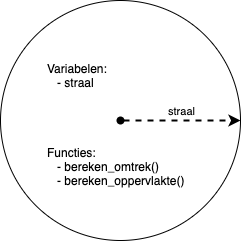
\includegraphics[scale=0.75]{Pictures/chapter07/cirkel.png}
% \caption{Ons cirkel-object heeft een straal, en kan (op basis daarvan) de omtrek en oppervlakte van zichzelf berekenen.}
% \label{fig:cirkel} % Unique label used for referencing the figure in-text
% %\addcontentsline{toc}{figure}{Figure \ref{fig:webserver}} % Uncomment to add the figure to the table of contents
% \end{figure}
%


% \newpage

% \section{Opdrachten}\index{Opdrachten}
% \begin{exercise}
% $\\$
% \end{exercise}

% \begin{exercise}
% $\\$
% \end{exercise}

% \begin{exercise}
% $\\$
% \end{exercise}

% \begin{exercise}
% $\\$
% \end{exercise}

% \begin{exercise}
% $\\$
% \end{exercise}

% \begin{exercise}
% $\\$
% \end{exercise}

% \begin{exercise}
% $\\$
% \end{exercise}

% \begin{exercise}
% $\\$
% \end{exercise}

